%------------------------------------------%
% Cannabis Data Science #84
% Copyright (c) 2022 Cannlytics
% Date: 9/21/2022
%------------------------------------------%
\documentclass[xcolor={dvipsnames}]{beamer}
\hypersetup{pdfpagemode = FullScreen}
\mode<presentation>{
  \usetheme{Boadilla}
  \usecolortheme{orchid}
  \usefonttheme{default}
  \setbeamertemplate{navigation symbols}{}
  \setbeamertemplate{caption}[numbered]
}
\setbeamersize{
  text margin left = 0.5in,
  text margin right = 0.5in
}

%------------------------------------------%
% Title
%------------------------------------------%
\title[\textbf{Cannabis Data Science \#84}]{}
\author{Cannlytics}
\institute[]{\Large Cannabis Data Science \#84}
\date{September \nth{21}, 2022}

%------------------------------------------%
% Packages
%------------------------------------------%
\usepackage[english]{babel}
\usepackage[utf8x]{inputenc}
\usepackage{tikz} % For styling.
\usepackage{xparse}
\usepackage{amsmath}
\renewcommand*\footnoterule{} % No footnote line.
\usepackage{mathtools} % Annotating equations.
\usepackage{hhline} % Double bars.
\usepackage[super]{nth} % 1st, 2nd, 3rd, etc.
\usepackage{graphicx, caption, subcaption}
\usepackage{setspace}
\usepackage[charter]{mathdesign}
\usepackage{tikz}
\usetikzlibrary{tikzmark}
\usetikzlibrary{arrows.meta}

%------------------------------------------%
% Theme
%------------------------------------------%
\definecolor{LG}{RGB}{218, 247, 166}
\definecolor{DG}{RGB}{2, 48, 32}
\setbeamercolor*{palette primary}{bg=LG, fg=DG}
\setbeamercolor*{palette secondary}{bg=LG, fg=DG}
\setbeamercolor*{palette tertiary}{bg=LG, fg=DG}

%------------------------------------------%
% Commands
%------------------------------------------%

% Top space.
\newcommand\T{\rule{0pt}{2.5ex}}

% Bottom space.
\newcommand\B{\rule[-1.25ex]{0pt}{0pt}}

% Blocks.
\newenvironment<>{Block}[2][.9\textwidth]
  {\setlength{\textwidth}{#1}
  \begin{actionenv}#3
    \def\insertblocktitle{#2}\par
    \usebeamertemplate{block begin}}
  {\par\usebeamertemplate{block end}
  \end{actionenv}}

% Balls.
\defbeamertemplate{enumerate item}{largeball}
{\begin{pgfpicture}{-1ex}{-0.65ex}{1.5ex}{1.5ex}
\usebeamercolor[fg]{item projected}
{\pgftransformscale{2.5}\pgftext{\Large\pgfuseshading{bigsphere}}}
{\pgftransformshift{\pgfpoint{0pt}{0.5pt}}
\pgftext{\usebeamerfont*{item projected}\small\insertenumlabel}}
\end{pgfpicture}}

% Fancy arrows.
\NewDocumentCommand\UpArrow{O{2.0ex} O{black}}{%
   \mathrel{\tikz[baseline] \draw [->, line width=0.5pt, #2] (0,0) -- ++(0,#1);}} % Fancy up-arrow.
\NewDocumentCommand\DownArrow{O{2.0ex} O{black}}{%
   \mathrel{\tikz[baseline] \draw [<-, line width=0.5pt, #2] (0,0) -- ++(0,#1);}} % Fancy down-arrow.

% Equations with numbers on the left.
\makeatletter
\newcommand{\LeftEqNo}{\let\veqno\@@leqno}
\makeatother

% Print out title.
\defbeamertemplate*{title page}{customized}[1][]
{
  \usebeamerfont{title}\inserttitle\par
  \bigskip
  \vspace{0.5\baselineskip}
  \usebeamerfont{institute}\insertinstitute\par
  \vspace{0.5\baselineskip}
  {\small\usebeamerfont{date}\insertdate\par}
  \usebeamercolor[fg]{titlegraphic}\inserttitlegraphic
}

%------------------------------------------%
% Presentation
%------------------------------------------%
\begin{document}

% Title page.
\begin{frame}{}

% Background
\tikz[remember picture, overlay]
\node[opacity=1.0, inner sep=0pt] at (current page.center){
  
\includegraphics[height=\paperheight, width=\paperwidth]{images/presentation-cover.pdf}
};

% Title
\vspace*{4\baselineskip}

\includegraphics[scale=0.375]{images/logo.pdf}
\vspace*{-2\baselineskip}
\titlepage
\end{frame}


\begin{frame}{}
\begin{minipage}{0.45\linewidth}
\vspace{-6\baselineskip}

% Quote
{\small ``Artificial selection is the process by which humans choose individual organisms with certain {\bfseries phenotypic} trait values for breeding. If there is additive \underline{genetic variance} for the selected trait, it will respond to the selection, that is, the trait will {\itshape evolve}.''}
\begin{flushright}
{\footnotesize
JK Conner, in Encyclopedia of Evolutionary Biology, 2016
}
\end{flushright}

\end{minipage}\hspace{0.045\linewidth}%
\begin{minipage}{0.45\linewidth}

% Image
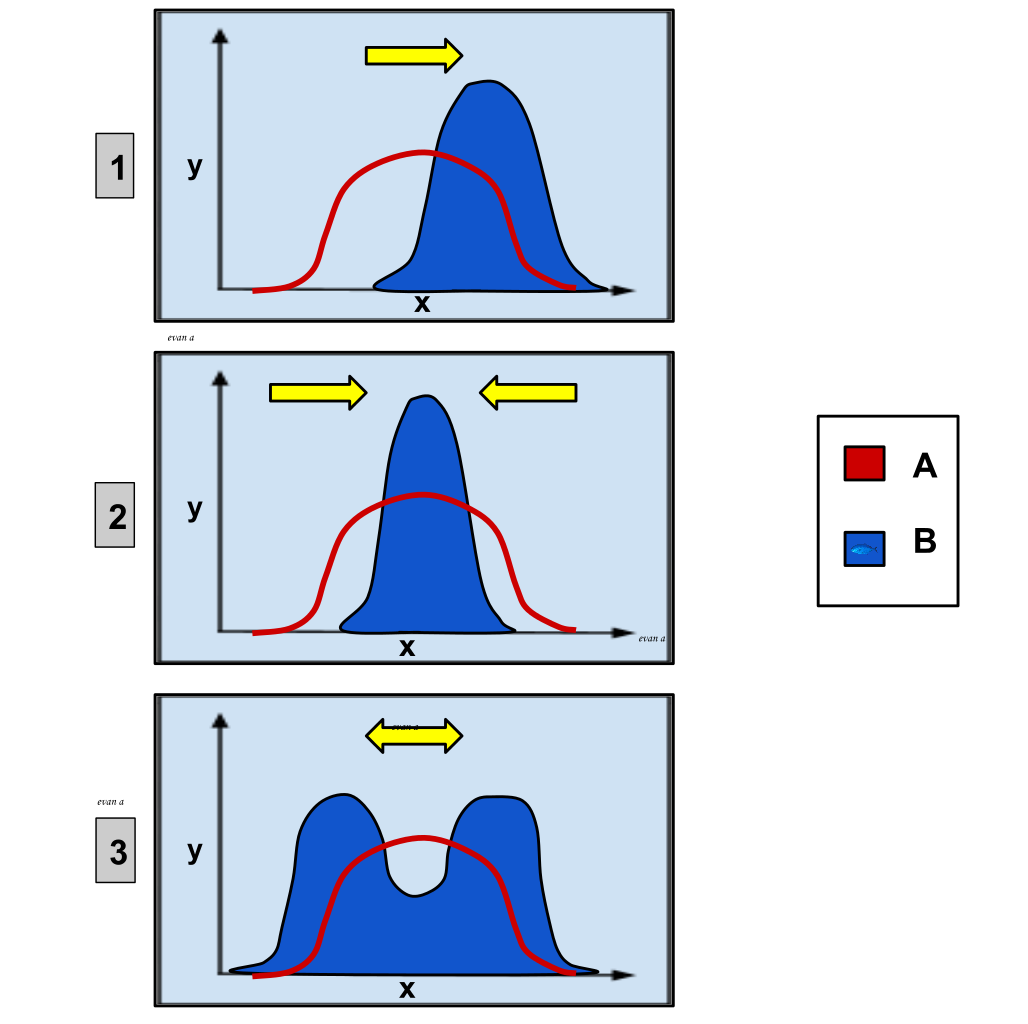
\includegraphics[width=2in]{images/genetic-distribution.png}
{\footnotesize
\begin{enumerate}
\item A single extreme phenotype is favored;
\item The intermediate phenotype is favored over the extreme traits;
\item The extreme phenotypes are favored over the intermediate.
\end{enumerate}
}
{\tiny
Author:  Ealbert17\\
License: CC BY-SA 4.0 \\
\texttt{https://creativecommons.org/licenses/by-sa/4.0}
}

\end{minipage}


\end{frame}


\begin{frame}{Relevant Topics in Biology}

\begin{itemize}

\item Artificial vs. natural selection;

\vspace{1\baselineskip}

\item Genetic drift;

\vspace{1\baselineskip}

\item Chemovars or chemoforms;

\vspace{1\baselineskip}

\item Plant cutting / cloning;

\vspace{1\baselineskip}

\item {\bfseries Pharming}!

\end{itemize}

\end{frame}


\begin{frame}{The Emergence of Cannabis Chemovars}
%
%Can we model strain emergence similar to a virus. For example, do certain strain names go viral or spread around the country?

%\begin{center}
\begin{minipage}{\textwidth}
\begin{Block}{Hypotheses}

\vspace{0.75\baselineskip}

\begin{itemize}

\item Can we find the data / producer / state of the \nth{1} ocurrance of a particular strain?

\vspace{0.75\baselineskip}

\item Can we find the date a particular strain spread to another state?

\vspace{0.75\baselineskip}

\item Do chemical profiles vary by region?

\vspace{0.75\baselineskip}

\item Does California cannabis show more chemical variation than in Michigan or Massachusetts?

\begin{itemize}

\footnotesize

\vspace{0.5\baselineskip}

\item Do new strains arise more often in CA than in MA because a larger proportion of plants are grown from seed versus clone?

\vspace{0.5\baselineskip}

\item Are concentrates more variable in CA than in MI or MA because of source flower?

\end{itemize}

\vspace{0.75\baselineskip}

\item 

\vspace{0.75\baselineskip}

\end{itemize}

\end{Block}
\end{minipage}

\end{frame}


%------------------------------------------%
% Optical Character Recognition (OCR)
%------------------------------------------%
%\begin{frame}{Early Optical Character Recognition (OCR)}
%
%% Optophone section
%\begin{minipage}{0.45\textwidth}
%
%\vspace{-6\baselineskip}
%\footnotesize
%
%\begin{itemize}
%
%\item 1914 - 1931: {\bfseries Emanuel Goldberg} created machines to read characters and convert them into standard telegraph code.
%
%\end{itemize}
%
%\end{minipage}\hspace{0.05\textwidth}%
%\begin{minipage}{0.45\textwidth}
%
%\vspace{1\baselineskip}
%\begin{figure}
%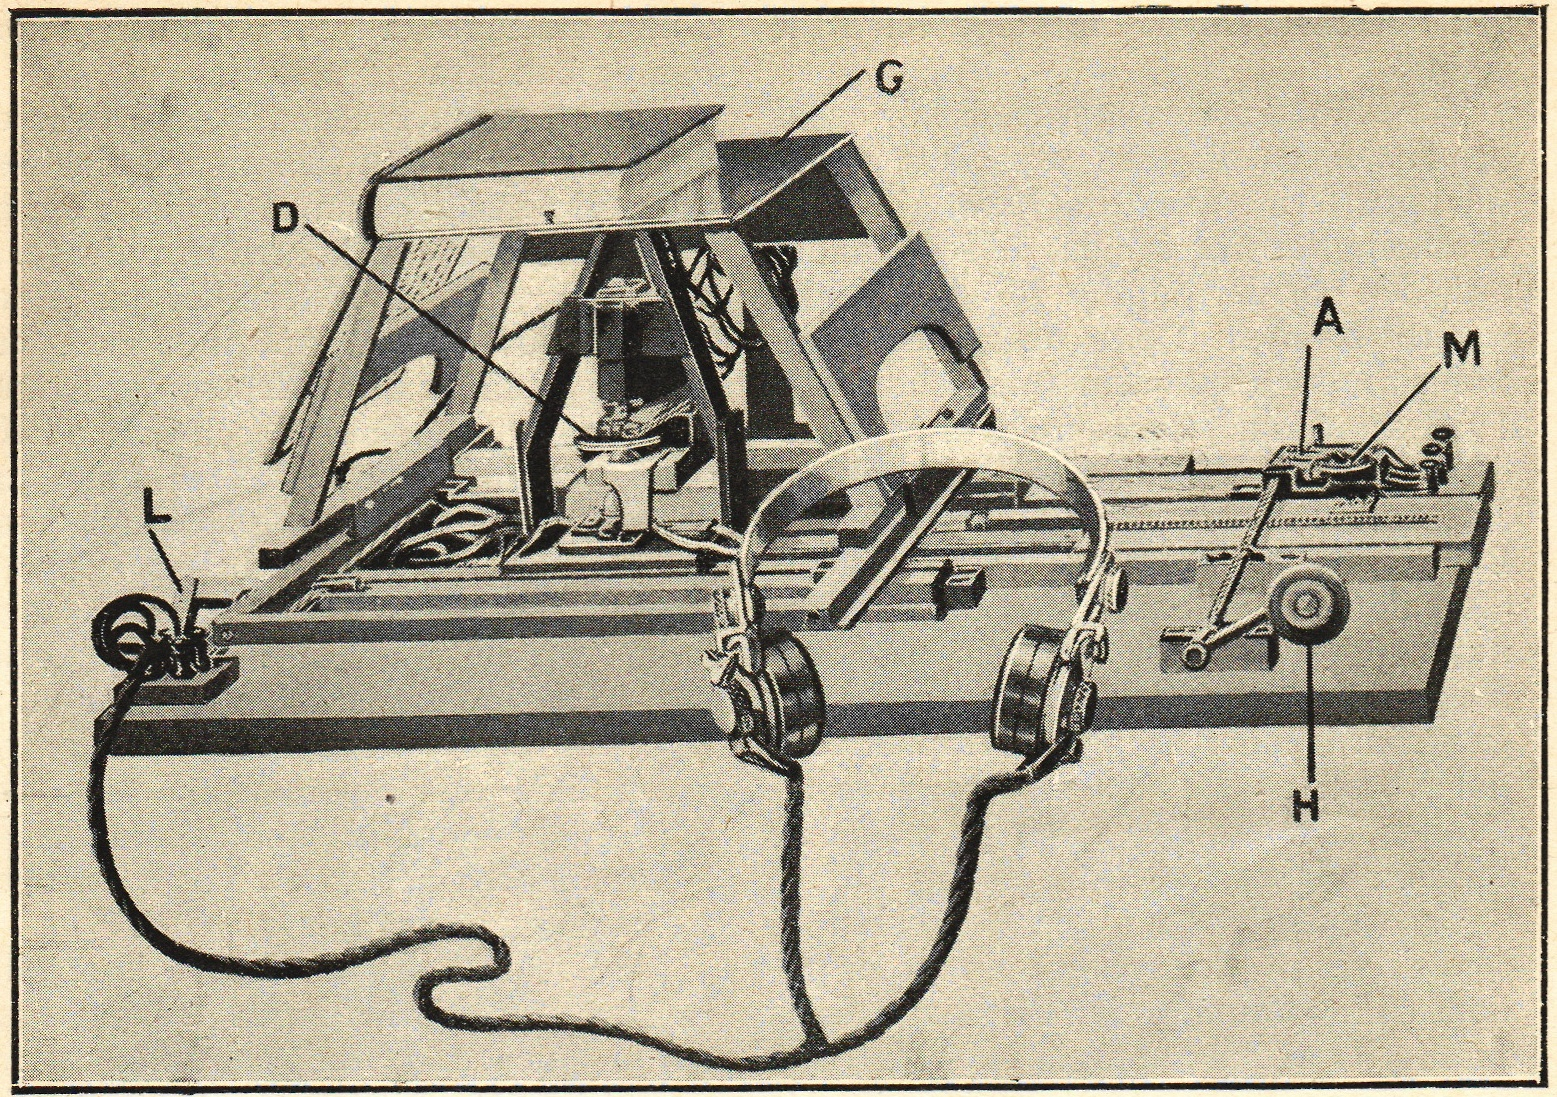
\includegraphics[width=\textwidth]{images/optophone.jpg}
%\caption*{\footnotesize An {\bfseries optophone}, scans text and generates time-varying chords of tones to identify letters.}
%
%\vspace{-0.5\baselineskip}
%{\tiny Note: Uses \underline{selenium} photosensors!}
%\end{figure}
%
%\end{minipage}
%
%
%% Ray Kurzweil section
%\begin{minipage}{0.45\textwidth}
%
%\vspace{-6\baselineskip}
%
%\begin{itemize}
%
%\footnotesize
%
%\item 1974: {\bfseries\footnotesize Ray Kurzweil} monetized OCR to recognize virtually any printed font.
%
%\end{itemize}
%
%\vspace{-0.5\baselineskip}
%\begin{figure}
%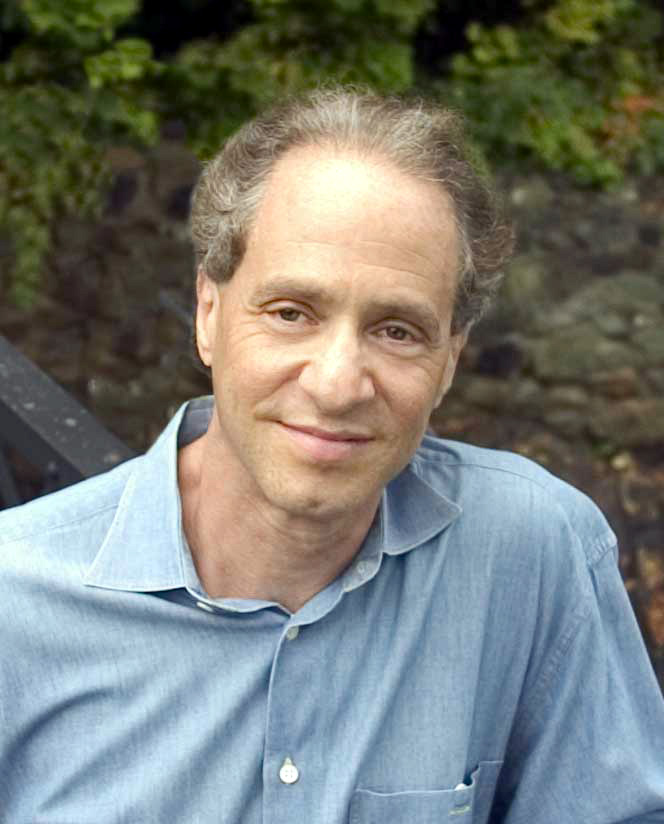
\includegraphics[width=0.55\textwidth]{images/kurzweil.jpg}\\
%{\tiny
%Photo by Michael Lutch \\
%License: CC BY 1.0 \\[-1\baselineskip]
%\texttt{https://creativecommons.org/licenses/by/1.0}
%}
%\end{figure}
%
%\end{minipage}\hspace{0.05\textwidth}%
%\begin{minipage}{0.45\textwidth}
%
%\footnotesize
%
%\vspace{-0.25\baselineskip}
%\begin{itemize}
%
%\footnotesize
%
%\item 1978: {\bfseries LexisNexis} parsed legal documents into online databases.
%
%\vspace{0.25\baselineskip}
%
%\item 2000s: First web-based OCR applications.
%
%\end{itemize}
%
%\end{minipage}
%
%\end{frame}


%------------------------------------------%
% Question of the Day
%------------------------------------------%

%\begin{frame}{Cannabis Data Science Application}
%
%\begin{center}
%\begin{minipage}{3.85in}
%
%% Thank you.
%
%\begin{center}
%\begin{minipage}{0.9\linewidth}
%\begin{Block}{Questions of the Day}
%
%\vspace{0.75\baselineskip}
%
%\begin{itemize}
%
%\item Can the data be extracted from a {\bfseries COA} image taken by a consumer at a retailer?
%
%\vspace{0.75\baselineskip}
%
%\item Given consumer's history, $\overline{X}$, can we predict product(s) with chemical profile(s), $\hat{Y}$, that the consumer may {\itshape enjoy}?
%
%\vspace{0.75\baselineskip}
%
%\end{itemize}
%
%\end{Block}
%\end{minipage}
%\end{center}
%
%\vfill
%
%\end{minipage}
%\end{center}
%
%\end{frame}


%------------------------------------------%
% Recommendation Engines
%------------------------------------------%

%\begin{frame}{Product Recommendation Algorithm}
%
%\vspace{0.5\baselineskip}
%Algorithm:
%
%\begin{enumerate}
%
%\small
%
%\vspace{0.75\baselineskip}
%\item Calculate average product concentrations by consumer, $\bar{X}$;
%
%\vspace{0.75\baselineskip}
%\item Find $k$-nearest products, $\hat{Y}$, given the average concentrations;
%
%\vspace{0.75\baselineskip}
%\item Repeat when the consumer makes a purchase.
%
%\end{enumerate}
%
%\vspace{1\baselineskip}
%
%Extension:
%
%\begin{itemize}
%
%\small
%
%\vspace{0.75\baselineskip}
%\item Weighted average by {\bfseries sentiment analysis}:
%
%$$
%\bar{X} = \frac{\sum_{m=1}^M \theta_m X_m}{\sum_{m=1}^M \theta_m},
%$$
%
%\vspace{0.75\baselineskip}
%where $\theta_m$ is a consumer's sentiment score (0 to 1) for a review of each product, $m$, of $M$ total products.
%
%\end{itemize}
%
%\end{frame}


% Note: This is a consumer-specific recommendation engine! This is awesome because we expect different people have different biochemistries and react differently to cannabis products.

%------------------------------------------%
% Takeaway
%------------------------------------------%
\section{Takeaway}

\begin{frame}{}

\vspace{0.5\baselineskip}

\begin{center}
\begin{minipage}{3.85in}

% Thank you.

\includegraphics[width=.25in]{images/prayer.png} {\Large \textbf{Thank you for coming.}}\\[-0.75\baselineskip]

\begin{center}
\begin{minipage}{0.75\linewidth}
\begin{Block}{Insights of the Day}

\vspace{0.5\baselineskip}

\begin{itemize}

\vspace{0.75\baselineskip}
\item Plant a seed: you never know what will grow.

\vspace{0.75\baselineskip}

\end{itemize}

\end{Block}
\end{minipage}
\end{center}

\vfill

\end{minipage}
\end{center}

\vspace{0.5\baselineskip}

{\large What is on your mind for next week?}\\

\end{frame}


%------------------------------------------%
% Fin.
%------------------------------------------%
\end{document}
